\subsection{Visitor Pattern}
\label{sec:VisitorDesign}

As can be seen on figure \ref{fig:CompilerProcess}, several steps in the compilation process acts on the AST, with semantic analysis containing both type- and borrow checking.
It would be desirable to have a unified way of traversing the structure for all the different steps. The immediate and naive solution would be to implement the different algorithms into the tree nodes directly. This approach has the appeal of making it easy to add new nodes. It does, however, make it difficult to add additional functionality to the compiler, as every addition requires a modification of every expression class. A solution to this great coupling is to use the visitor design pattern.

The visitor pattern separates algorithms from an object structure by implementing a 'visitor' class which can traverse the tree and perform the correct operations on each node. This allows for additional functionality to be added, without modifying the existing tree (thus following the open-closed principle). As long as every node implements an 'accept' function, new visitors can be added without the need for altering the expression classes at all. 

\begin{figure}
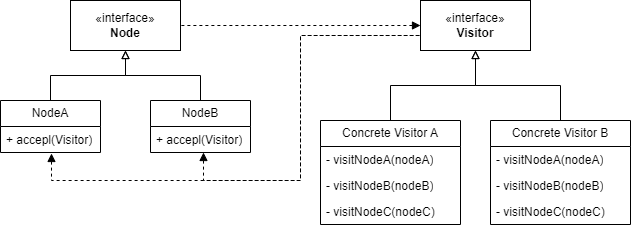
\includegraphics[width=\textwidth]{02-Body/Images/VisitorClassDiag.png}
\caption{Class diagram for Visitor Pattern}
\label{fig:VisitorClassDiagram}
\end{figure}